\documentclass{article}
\usepackage[utf8]{inputenc}
\usepackage{amsmath}
\usepackage{amsfonts}
\usepackage{amssymb}
\usepackage{minted}
\usepackage{titlesec}
\usepackage[a4paper,margin=1in,footskip=0.25in]{geometry}
\usepackage{fancyhdr}
\usepackage{graphicx}
\usepackage{float}
\pagestyle{fancy}
%basic page layout

\newcommand{\hwnumber}{6}
%header and footer settings
\lhead{Gen IMS II Homework \hwnumber}
\chead{Yiping Deng}
\rhead{\today}

\titlelabel{\thetitle\enspace}

\begin{document}
\title{Gen IMS II Homework \hwnumber}
\author{Yiping Deng}
\maketitle
\thispagestyle{fancy}
\section*{Task 1}
First, the transfer function
$$G(s) = \frac{R}{\frac{1}{C s} + R} = \frac{R C s}{1 + R C s}$$
Plug-in the wave input $j w$, we have:
$$G(j \omega) = \frac{R C \omega j}{1 + R C \omega j}$$
Then we calculate the norm to find out the change in magnitude:
\begin{align*}
    \| G(j \omega) \|^2 &= \| \frac{R C \omega j(1 - R C \omega j)}{1 + R^2 C^2 \omega^2} \|^2\\
    &= \frac{R^2 C^2 \omega^2}{1 + R^2 C^2 \omega^2} \\
	\| G(j \omega) \| &= \frac{R C \omega}{\sqrt{1 + R^2 C^2 \omega^2}}
\end{align*}
This implies that
$$\lim_{\omega \to \infty} \|G(j \omega)\| = 1$$
$$\lim_{\omega \to 0} \|G(j \omega)\| = 0$$
We can now use Matlab to plot this function:
\begin{figure}
\begin{minted}{matlab}
%% initial condition
R = 1e3;
C = 1e-6;
syms omega;
%% normal plot
fplot(log10(omega), 20 * log10(sqrt((R^2 * C^2 * omega^2)/(1 + R^2 * C^2 * omega^2))), [0.001, 100000])
hold on
fplot(20 * log10(1))
fplot(20 * log10(0.0000001))
hold off
%% end of file
\end{minted}
    \caption{Code for ploting Task 1}
\end{figure}
\begin{figure}[H]
    \centering
    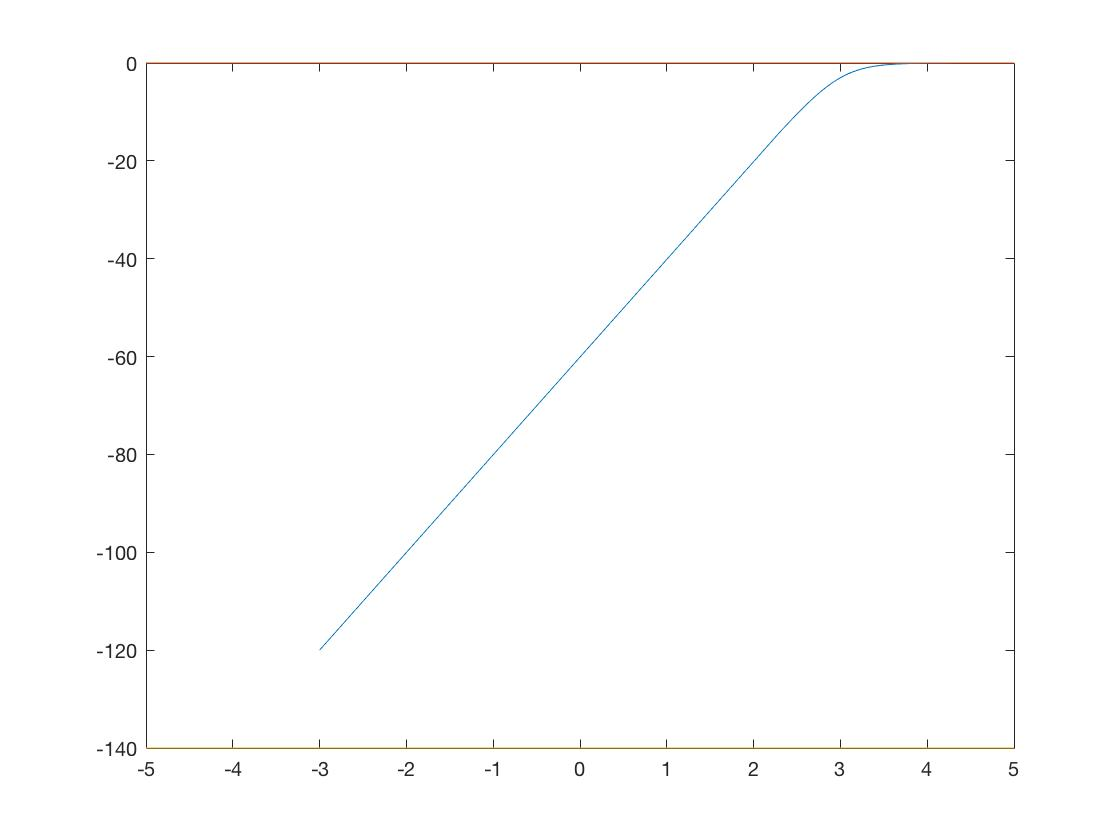
\includegraphics[width=\textwidth]{task1.jpg}
    \caption{Plot of $\| G(jw) \|$}
\end{figure}
\section*{Task 2}
First, the transfer function
$$ G(s) = \frac{\frac{1}{C s}}{R + \frac{1}{C s}} = \frac{1}{1 + R C s}$$
Then, you have
$$ \|G(j \omega)\| = \| \frac{1}{1 + R C \omega j} \| = \frac{1}{\sqrt{1 + R^2 C^2 w^2}}$$
Using the following Matlab code, have
\begin{figure}
\begin{minted}{matlab}
%% initial condition
R = 1e3;
C = 1e-6;
syms omega;
%% normal plot
fplot(log10(omega), 20 * log10(1 / sqrt(1 + R^2 * C^2 * omega^2)), [0.001, 100000])
hold on
fplot(20 * log10(1))
fplot(20 * log10(0.00001))
hold off
%% end of file
\end{minted}
\caption{Code for ploting Task 2}
\end{figure}
\begin{figure}[H]
    \centering
    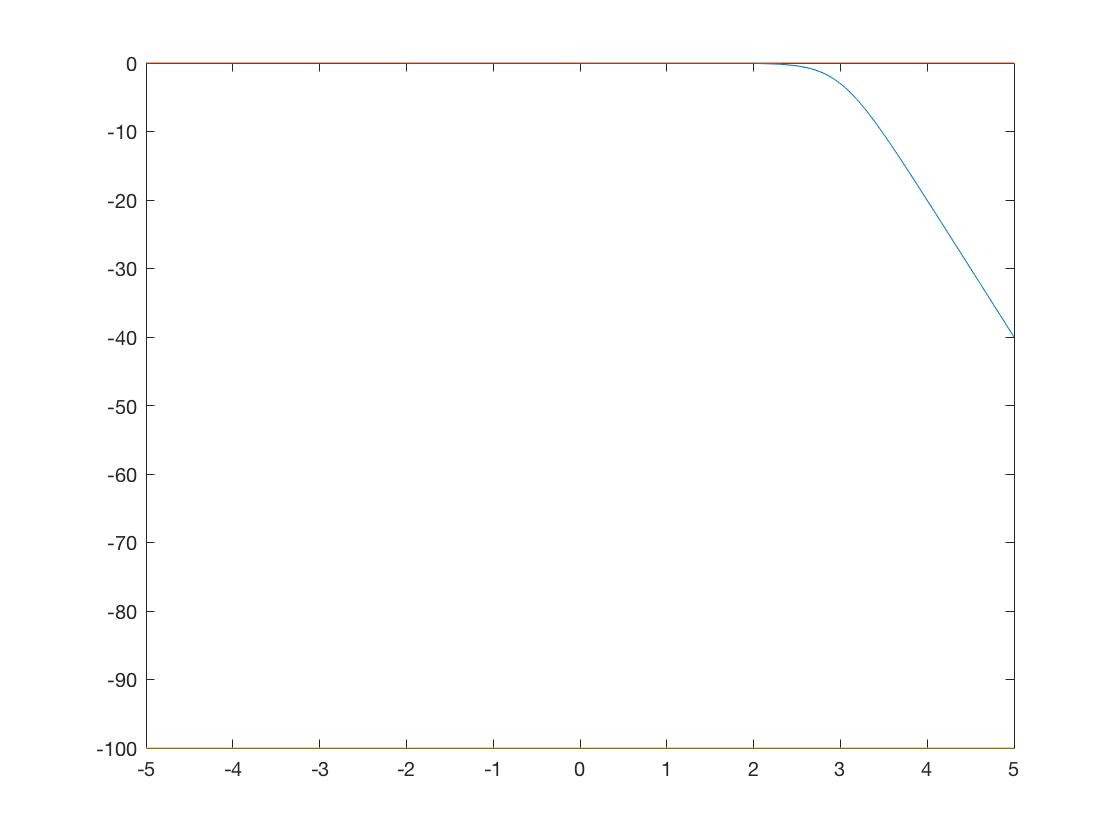
\includegraphics[width=\textwidth]{task2.jpg}
    \caption{Plot of $\| G(jw) \|$}
\end{figure}
\section*{Task 3}
From the above solution, we have
$$\|G_{band}(j \omega)\| = \|G_{high}(j \omega)\| \cdot \|G_{low}{j \omega} \| $$
Using the Matlab code, we have
\begin{figure}[H]
    \begin{minted}{matlab}
        %% initial condition
        R = 1e3;
        C = 1e-6;
        syms omega;
        %% normal plot
        fplot(log10(omega), 20 * log10(1 / sqrt(1 + R^2 * C^2 * omega^2) * sqrt((R^2 * C^2 * omega^2)/(1 + R^2 * C^2 * omega^2))), [0.01, 5000])
        hold on
        fplot(20 * log10(1))
        fplot(20 * log10(0.00001))
        hold off
        %% end of file
\end{minted}
\caption{Code for Task3}
\end{figure}
\begin{figure}[H]
    \centering
    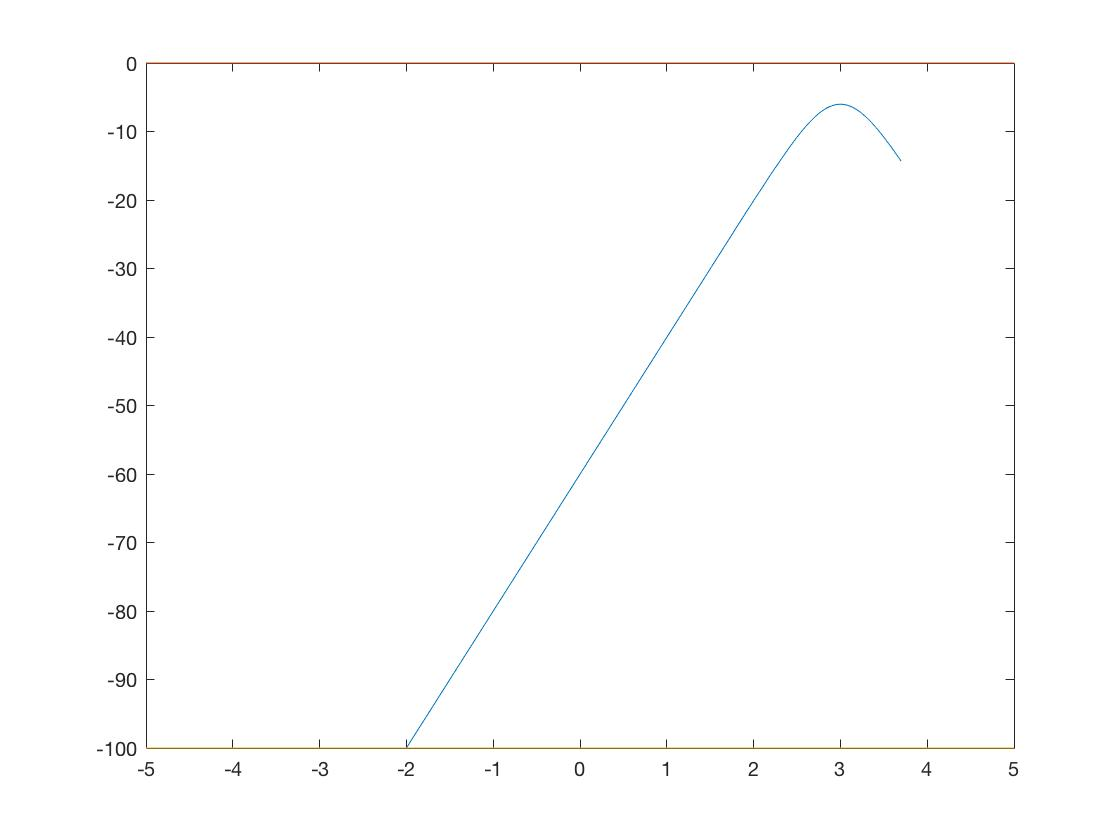
\includegraphics[width=\textwidth]{task3.jpg}
    \caption{Plot of $\| G(jw) \|$}
\end{figure}

\end{document}
